\subsection{}
\begin{tabular}{lll}
literal & int & long \\
\hline
binary & /0b[0-1]+/ & /0b[0-1]+(l|L)/ \\
octal & $ /0(0|[1-7][0-7])+/ $ & /0(0|[1-7][0-7])+(l|L)/ \\
hexadecimal & $ /0x[0-9a-f]+/ $ & $ /0x[0-9a-f]+(l|L)/ $ \\
decimal & $ /(0|[1-9][0-9]*)/ $ & $ /(0|[1-9][0-9]*(l|L))/ $ \\
\end{tabular}
\subsection{}
\begin{figure}[H]
\centering
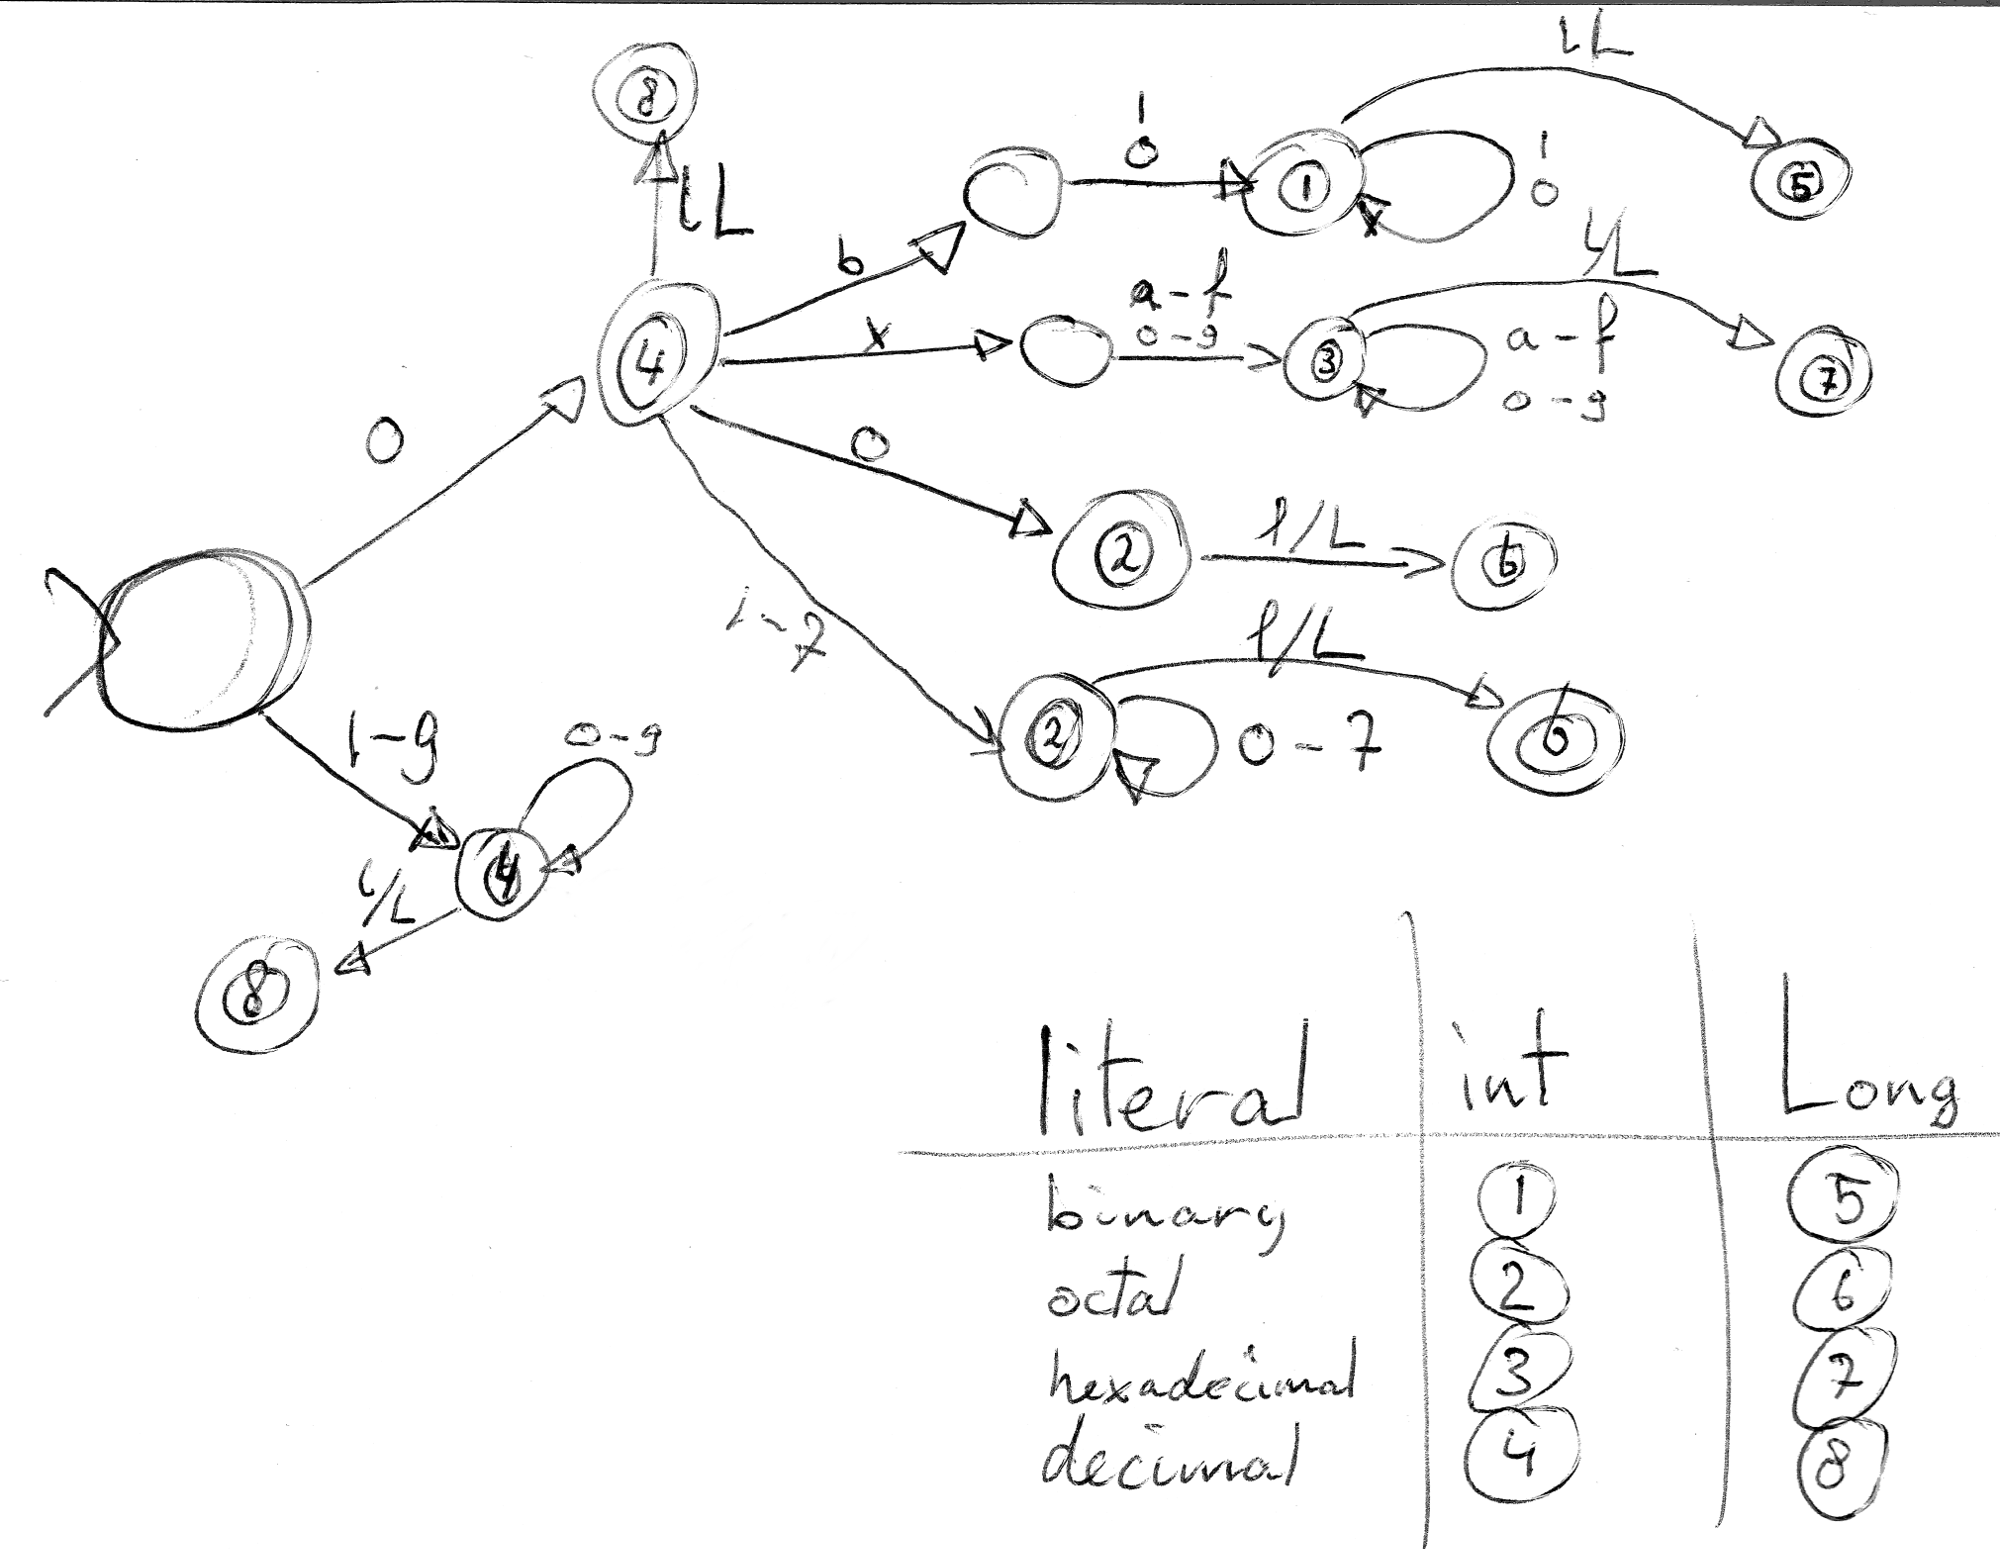
\includegraphics[width=\linewidth]{2_small.png}
\caption{A DFA combining the token types}
\end{figure}
\subsection{}
See the code in \texttt{pp.s1378791.q1\_2.Numbers.g4} and \texttt{pp.s1378791.q1\_2.NumbersTest}